\documentclass{article}

% If you're new to LaTeX, here's some short tutorials:
% https://www.overleaf.com/learn/latex/Learn_LaTeX_in_30_minutes
% https://en.wikibooks.org/wiki/LaTeX/Basics

% Formatting
\usepackage[utf8]{inputenc}
\usepackage[margin=1in]{geometry}
\usepackage[titletoc,title]{appendix}
\usepackage{hyperref}

% Math
% https://www.overleaf.com/learn/latex/Mathematical_expressions
% https://en.wikibooks.org/wiki/LaTeX/Mathematics
\usepackage{amsmath,amsfonts,amssymb,mathtools}

% Images
% https://www.overleaf.com/learn/latex/Inserting_Images
% https://en.wikibooks.org/wiki/LaTeX/Floats,_Figures_and_Captions
\usepackage{graphicx,float}

% Tables
% https://www.overleaf.com/learn/latex/Tables
% https://en.wikibooks.org/wiki/LaTeX/Tables

% Algorithms
% https://www.overleaf.com/learn/latex/algorithms
% https://en.wikibooks.org/wiki/LaTeX/Algorithms
\usepackage[ruled,vlined]{algorithm2e}
\usepackage{algorithmic}

% Code syntax highlighting
% https://www.overleaf.com/learn/latex/Code_Highlighting_with_minted
\usepackage{minted}
\usemintedstyle{borland}

% References
% https://www.overleaf.com/learn/latex/Bibliography_management_in_LaTeX
% https://en.wikibooks.org/wiki/LaTeX/Bibliography_Management
\usepackage{biblatex}
\addbibresource{references.bib}

% Title content
\title{Statistical Physics - Paris Physics Master\\
    Home exercices - Solution}
\author{David L. Paipa}
\date{November 2020}

\begin{document}

\maketitle

% Abstract
% \begin{abstract}
%     Add your abstract here.
% \end{abstract}

% Introduction and Overview
\section{Random Walk}

% Example Subsection
\subsection{Displacement}
\textit{
Consider a random walk in three dimensions: each step is a vector whose components are three random numbers uniformly distributed in the interval $[-a;+a]$ (x; y components) or $[d -a; d + a]$ (z component), with $a > 0$. What are the average displacement and the mean squared displacement after N steps? Explain your calculations, and propose a possible physical system that could be modelled in this way.}


% Example Subsubsection
\subsection*{Solution}

\subsubsection*{position after N steps}
First lets show the expected value of the position for each of the axes i.e. $\langle n_x\rangle ,\langle n_y \rangle,\langle n_z\rangle$. It is known that the deduction process for X-axis is the same as for Y-axis, since when adding a new step $x_i$ to the random walk they use the same distribution of values $P(n)$. I asume the walk walk starts at the coordinates $(0, 0, 0)$\\

Lets denote $\langle n_x \rangle_N$ the X position of the walker at the step $N$, being this equivalent to:
\begin{equation}
\langle n_x \rangle_N = \langle \sum_{i=1}^N x_i \rangle = \sum_{i=1}^N \langle  x_i \rangle
\end{equation}

Where each $x_i$ is taken from a uniform distribution in the range $[-a,a]$ . As each $x_i$is uncorrelated with $x_j$ if $i \neq j$, is true that
\begin{equation}
    \langle n_x \rangle_N = N \langle x_i \rangle
\end{equation}

We can asume that a value $\ell$ is taken suchthat $0 \leq \ell \leq a$ and that $- \ell$ is equally probable in the given distribution for any $\ell$. Then, $P(x_i = -\ell) = P(x_i = \ell) = 1/2$ and therefore,

\begin{equation}
    \langle x_i \rangle = \sum_{k} p_k x_k = \frac{1}{2}(-\ell) + \frac{1}{2}(\ell) = 0 \quad \forall \ell \in [0,a]
\end{equation}

where $p_k$ is the probability associated with the outcome $x_k$. Since this happens for any $\ell$ magnitude in the given interval , I conclude $\langle x_i \rangle = 0$ . Then,

\begin{equation}
     \langle n_x \rangle_N = \langle n_y \rangle_N = 0
\end{equation}

For $\langle n_z\rangle$ the distribution for every new step is different. We use the same element of random magnitude $\ell$ within the same ranges $0 \leq \ell \leq a$ (behaving as $\langle x_i \rangle$), but this time we add a constant factor $d$. We can say that,

\begin{equation}
   \langle n_z \rangle_N =\langle \sum_{i=1}^N z_i \rangle = \langle \sum_{i=1}^N   d + x_i \rangle = \sum_{i=1}^N d + \langle x_i \rangle
\end{equation}

Since each $z_i$ is equally independent form $z_j$ when $i \neq j$, then its true that
\begin{equation}
    \langle n_z \rangle_N = N \left( d + \langle x_i \rangle \right) = Nd
\end{equation}


Given the previous definitions I can conclude that
\begin{equation}
\langle \vec{r} \rangle_N = (0,0,Nd)   
\end{equation}
These conclusions can be compared with simulations on a random walk using the rules shown previously. The results observed agree with the theory .

\begin{figure}[h]
\centering
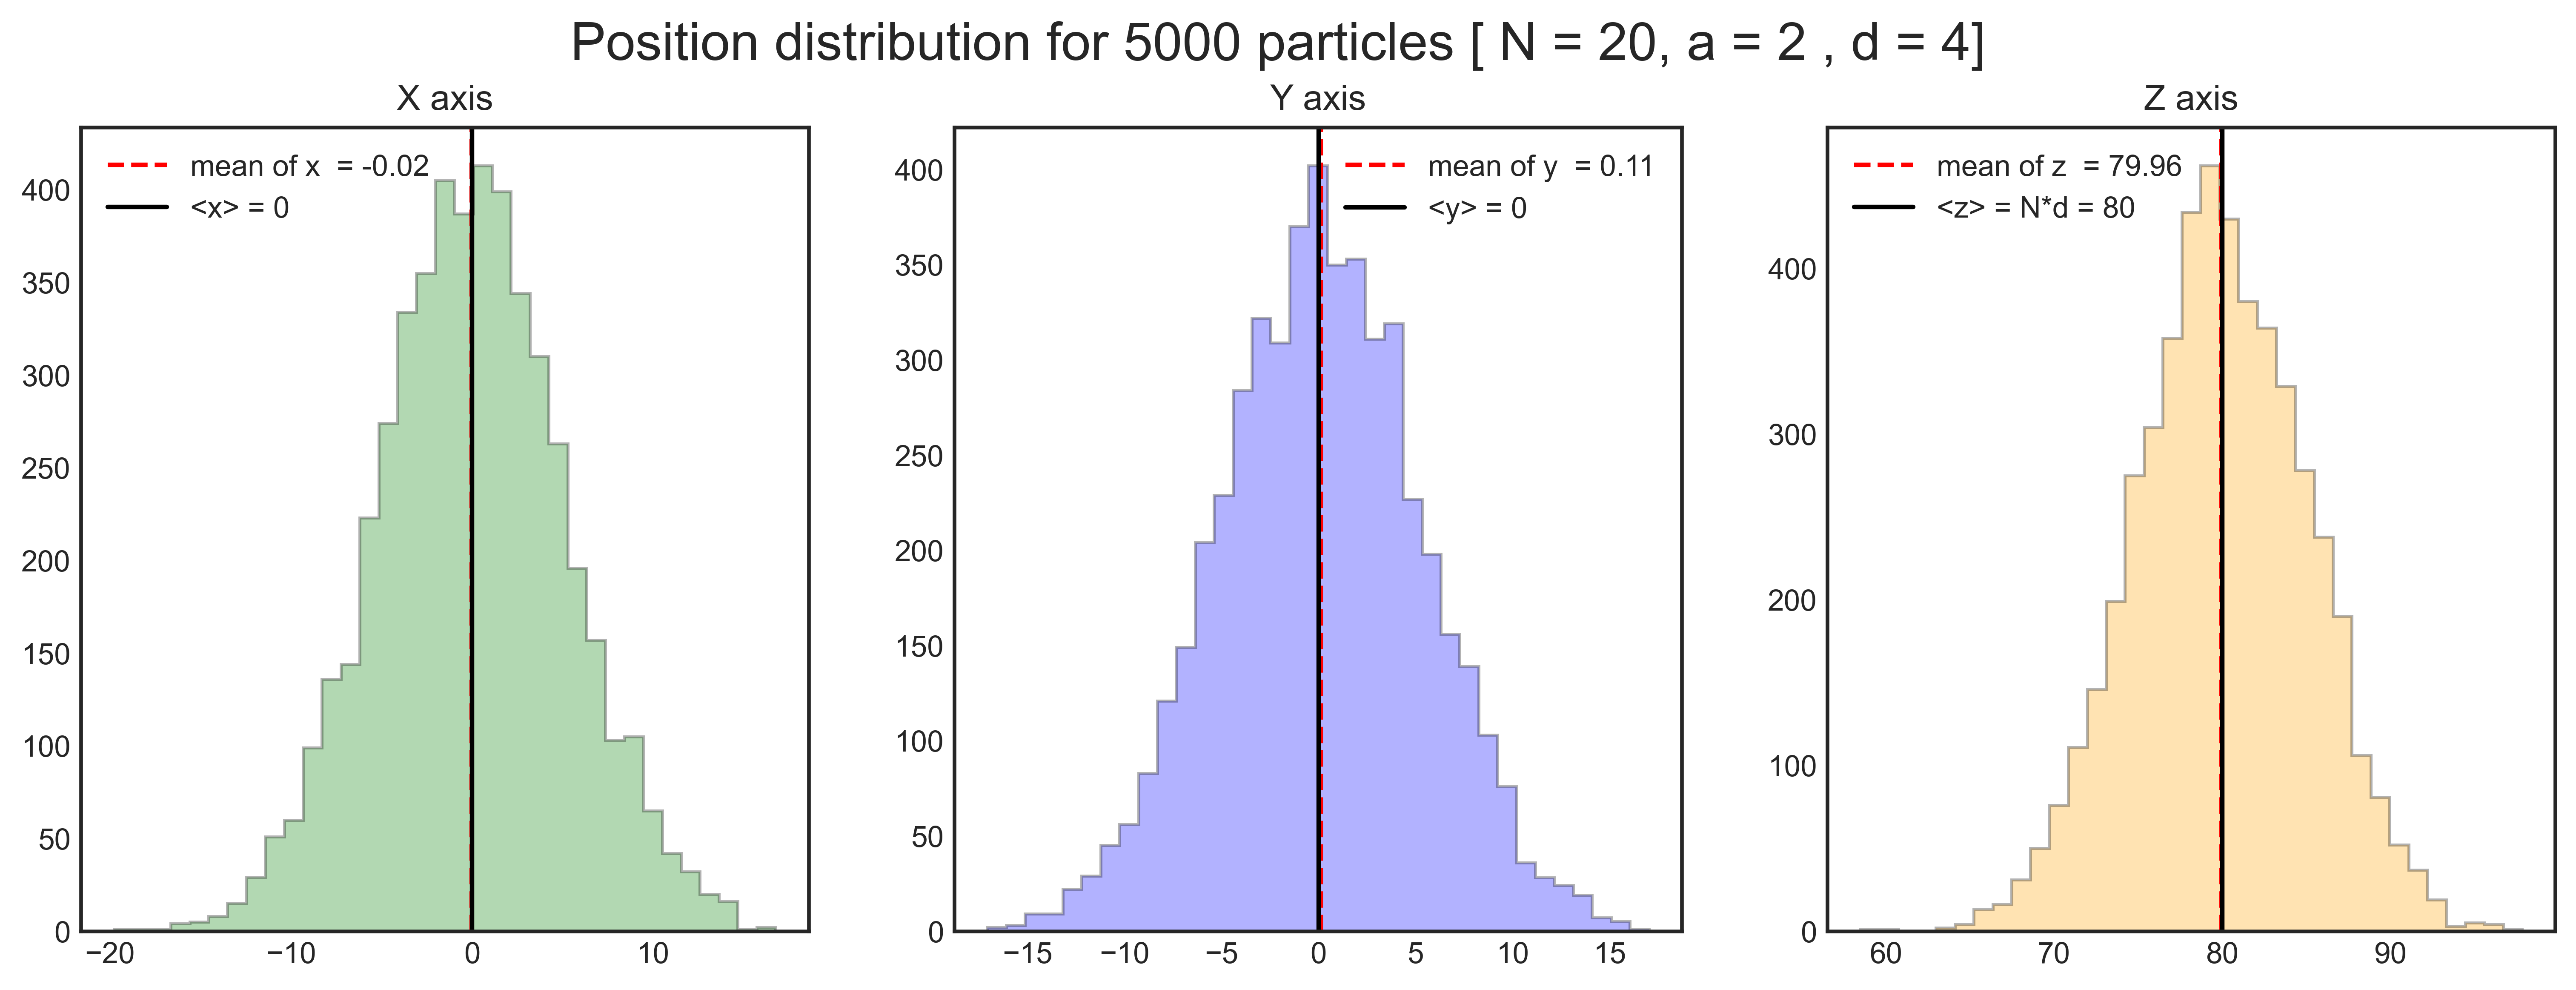
\includegraphics[width=1\textwidth]{imgs/pos_randomwalk.png}
\caption{Random walk in each axis showing the final position of the walkers after N steps, the mean value obtained by the simulation in each axis and the analytically inferred expected value.}
\end{figure}


\subsubsection*{Mean squared position}

For the mean squared displacements in each axes I will use an integral solution.  I denote the mean squared displacements as $\langle n_x^2\rangle ,\langle n_y^2 \rangle,\langle n_z^2\rangle$. Again, I will asume the solution for  $\langle n_x^2\rangle$ also applies for $\langle n_y^2\rangle$. By definition,

\begin{equation}
    \langle n_x^2\rangle_N = \langle \left(\sum_{i=1}^N x_i\right)^2 \rangle = \langle \sum_{i=1}^N x_i^2 + \sum_{i=1}^N \sum_{\substack{j=1\\i\neq j}}^N x_i x_j \rangle = N \langle x_i^2 \rangle 
\end{equation}

Using the argument that each $x_i$ is an independant variable, it is true that  $\langle x_i x_j \rangle = 0 $ for $i \neq j$. For the value of $\langle x_i^2\rangle$ we have that
\begin{equation}
    \langle x_i^2\rangle =  \int_{-a}^{a} x_i^2 P(x_i) dx = \frac{1}{2a} \left[ \frac{x_i^3}{3} \right]_{-a}^{a} = \frac{2a^3}{6a} = \frac{a^2}{3}
\end{equation}
Note that the factor $(2a)^{-1}$ is the probability $P(x_i)$ for each outcome in the interval $[-a,a]$ , since the accumulated probability in the interval should be 1. Therefore,

\begin{equation}
    \langle n_x^2\rangle_N =\langle n_y^2\rangle_N = N\frac{a^2}{3}
\end{equation}

Notice that the variance of  $n_x$ matches with the variance of the uniform distribution, which states that for a distribution of uniform probability (normalized) in an interval of length $\ell$ the variance is

\begin{equation}
    Var(U)_{\ell} = \frac{\ell^2}{12}
\end{equation}

In the case of $n_x$ (and by extension, also applies for $n_y$) we have that
\begin{equation}
Var(n_x) = \langle n_x^2 \rangle - \langle n_x \rangle^2 = \langle n_x^2 \rangle = \frac{a^2}{3}  = \frac{(2a)^2}{12} 
\end{equation}

For $ \langle n_z^2 \rangle_N$ I used a different approach. We start from the definition of the variance of $n_z$ ,which is also the same variance of $n_x$ and $n_y$. This can be inferred from the fact that the displacement of the sampling around the mean value is the same (a) and it  uses the same distribution to sample (Uniform distribution). Then,

\begin{equation}
    Var(n_z)_N = N\frac{a^2}{3}  =\langle n_x^2 \rangle_N - \langle n_z \rangle^2_N 
\end{equation}

From the previous expression\footnote{We can asume that the variance of a sum of random variables is equal to the sum of the variances since the term asociated with the covariance is canceled due to the argument of idependency. This allows the multiplication of the variance by N for the sum of N idependent outcomes.} we can infer the value of $\langle n_z^2 \rangle$ as

\begin{equation}
    \langle n_z^2 \rangle_N = Var(n_z)_N + \langle n_z \rangle^2_N = N\frac{a^2}{3} + (Nd)^2
\end{equation}

\begin{figure}[h]
\centering
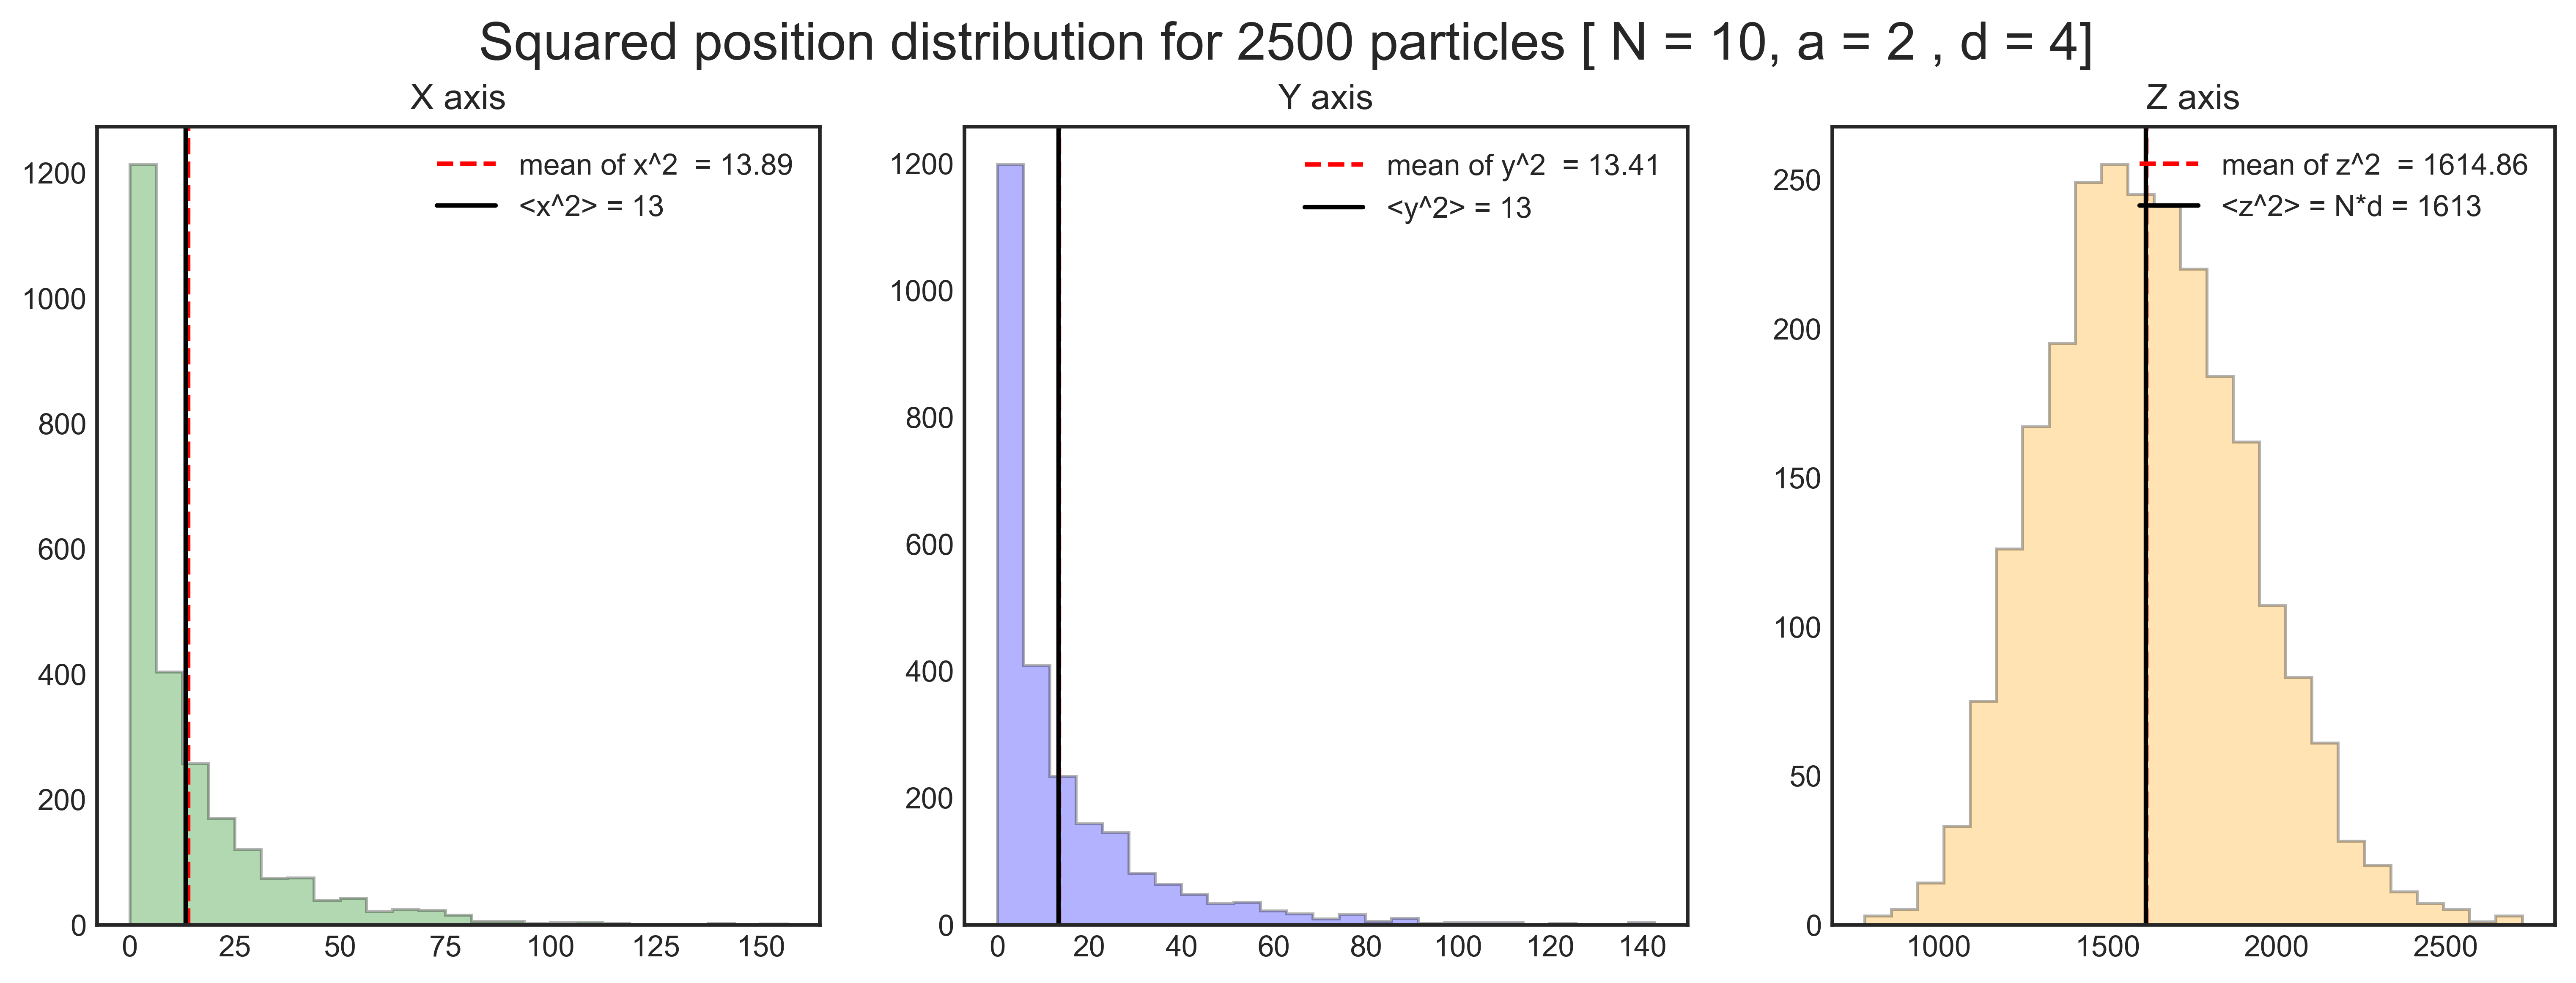
\includegraphics[width=1\textwidth]{imgs/pos2_randomwalk.png}
\caption{ The mean value of the squared displacement obtained by the simulation in each axis and the analytically inferred expected value.}
\end{figure}

the mean squared displacement is given by

\begin{equation}
    \langle \vec{r}^2 \rangle_N = <n_x^2>_N + <n_y^2>_N + <n_z^2>_N = Na^2 + (Nd)^2
\end{equation}
Then
\begin{equation}
    <D> = \sqrt{ \langle \vec{r}^2 \rangle_N} = \sqrt{Na^2 + (Nd)^2}
\end{equation}
We can verify these values with the simulated walks mentioned previously. 

\begin{figure}[h]
\centering
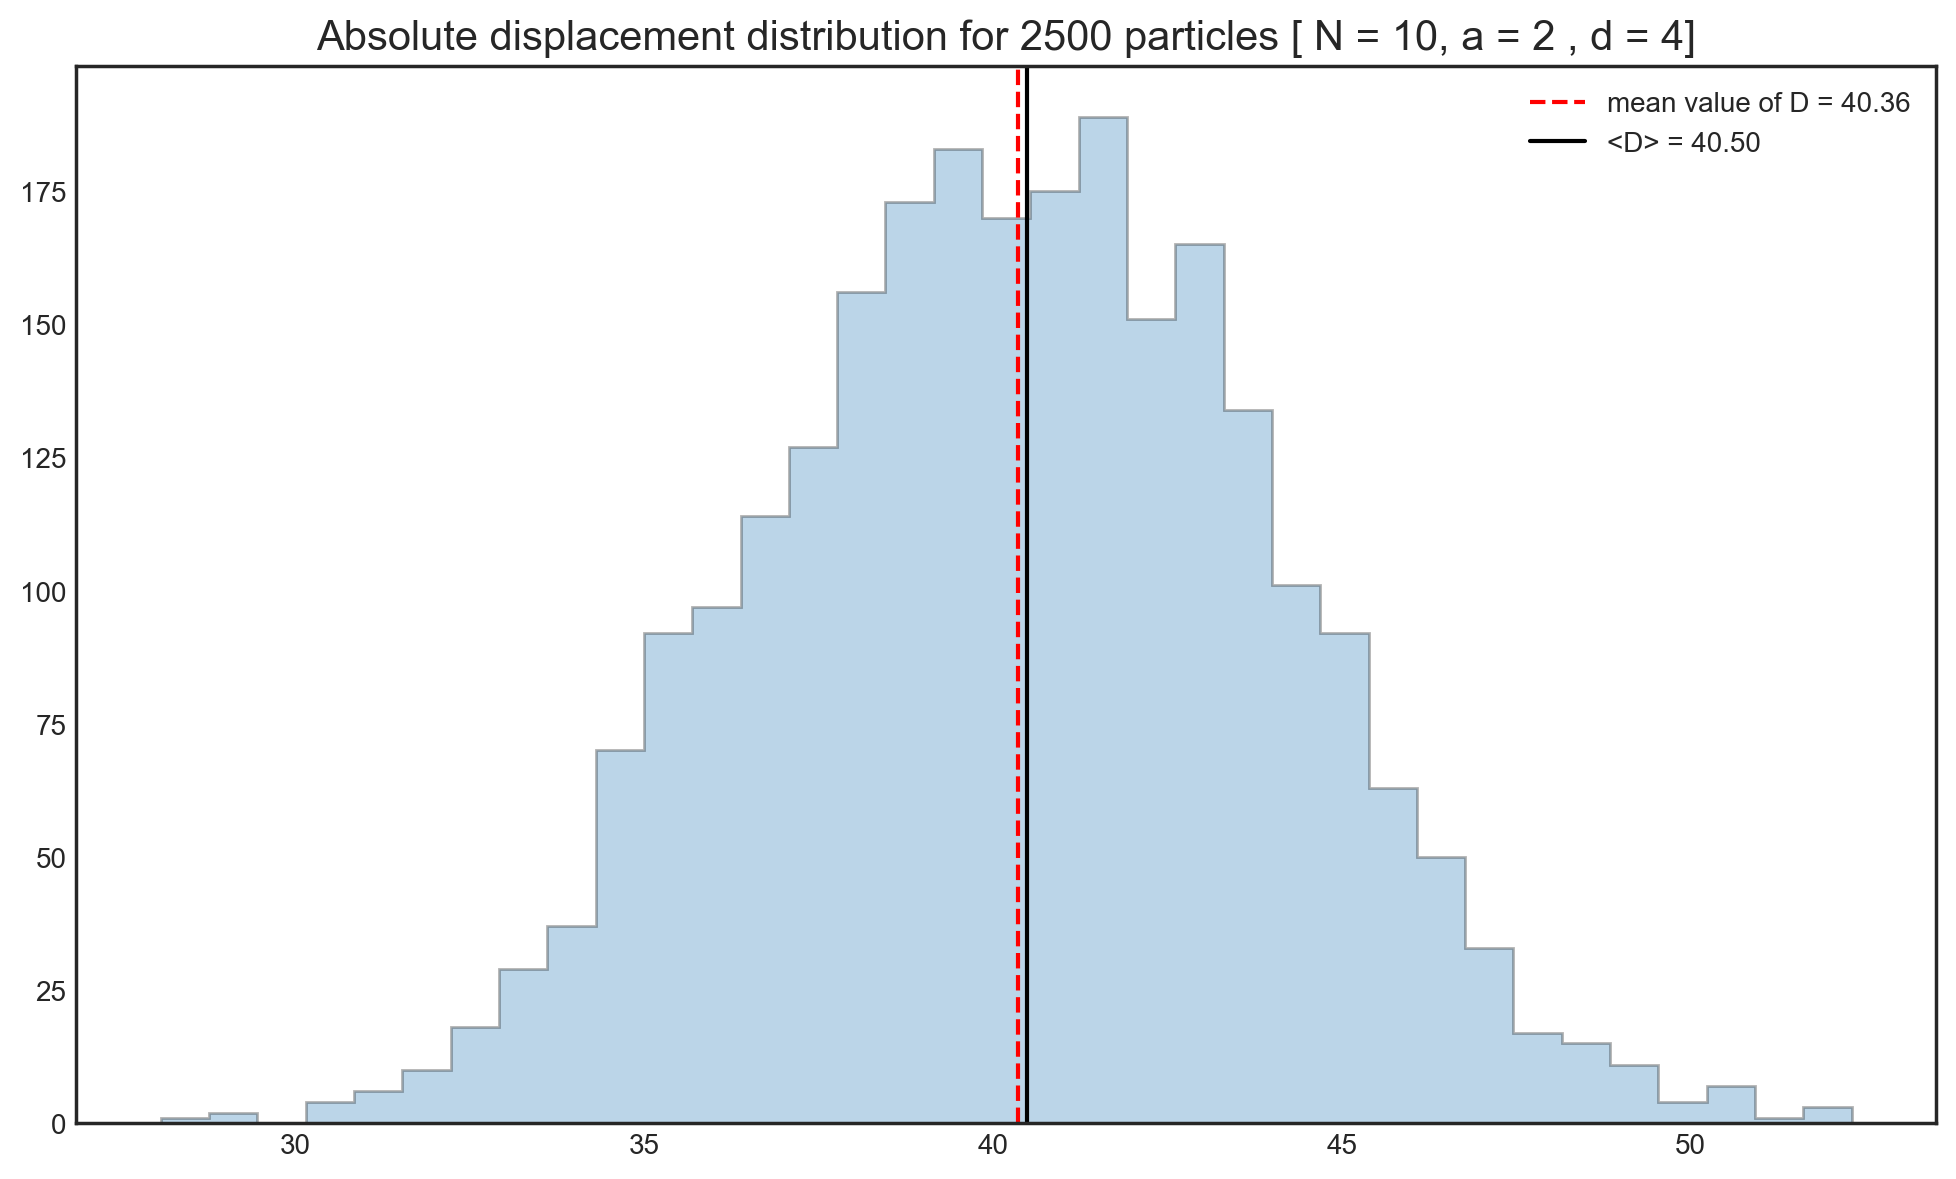
\includegraphics[width=0.7\textwidth]{imgs/d_randomwalk.png}
\caption{ The value of the root mean squared displacement i.e. the squared root of the mean squared distance.}
\end{figure}

When looking to the walks in Figure \ref{img:walks} we can observe difussion phoenomena in an isotropic medium (given that fluctioations in al three dimensions are of the same magnitude $a$) but with a aditional constant displcement in one of the three spatial dimensions. This can be compared  to physical systems such as a drop of ink (or any pullutant) diluting in a solvant under the influence of gravity. Another good example could be smoke originated in a point and spreading upwards due to convection of hot air.  

\subsection{Central Limit Theorem}
\textit{Explain what we can infer about the long-time displacement of a molecule in a liquid from the central limit theorem, without knowing the detailed interatomic forces. Can we apply the same reasoning to an impurity atom in a solid?}

\subsection*{Solution}
The central Limit Theorem states that the sum (normalized) of many \textbf{independent random variables} tends to a normal distribution even if the distribution from which the random variables come does not have Gaussian properties. This scenario can be seen in the random walks, or Brownian movement, since these are precisely the result of the sum of many random outcomes from the same distribution\footnote{More generalized representations of the theorem state that the sum of random variables of different distributions (different mean and variance) can also be represented with this theorem. The necessary condition is that both the mean and the variance of the distributions are finite.}. After a long time and with enough particles subject to Brownian motion, it is easy to show that the trend is towards a normal distribution. In the case studied, it can be observed in the position distributions in each of the axes and the RMS displacement distribtuion that the central limit theorem applies.

The displacement of a molecule in a liquid is describable under the phenomenon of Brownian motion. This is because the molecule is constantly colliding with the molecules of the liquid solvent, bouncing and traveling an arbitrary small distance in an equally random direction. If the solvent is isotropic and homogeneous, these displacements are not biased towards any direction or conditioned by any intensive property of the liquid itself. The latter is inferred since changing properties such as density or viscosity of the fluid would only affect the average distances of these small displacements and the frequency in which they happen, but would leave the nature of the random walk of the molecule in the solvent invariant. The homogeneous medium ensures that in a medium without any type of external potential (for example, gravity) for any arbitrary vector $\vec{r}$ of displacement, the vector $-\vec{r}$ is just as probable and therefore for a long period of time the limit theorem central applies to describe the stochastic process.\\

A solid is a structure organized in static lattices of atoms or ions that are only allowed to vibrate in these networks, transmitting specific frequencies in oscillations without changing places within the lattice. The Brownian phenomenon cannot explain the motion of an impurity within a solid mainly because, other than being fixed positions within the lattice, these vibrations depend on interatomic forces, and these forces do not necessarily have to be spatially isotropic.

\section{Partition functions}
\subsection{Electric polarization}
\textit{Calculate the electric polarization \textbf{P} of an ideal gas, consisting of molecules having a constant electric dipole moment $p$ in a homogeneous external electric field \textbf{E} at temperature $T$. What is the dielectric constant of this gas at small fields?}
\subsection*{Solution}
\subsubsection*{Polarization}
First lets remember the relation between the thermodinamic potentials and the Free energy of the system:
\begin{equation}
    dF(E,T,V) =  -PdV-SdT-\textbf{P}d\textbf{E} 
\end{equation}
Where the polarization \textbf{P} is given by
\begin{equation}
    \textbf{P} = -\frac{dF}{d\textbf{E}}
\end{equation}
But the definition of free energy is given by the partition function for the ensemble of $N$ particles subject to the electric field in question. It is important to bear in mind that these particles for now are punctual and do not have kinetic energy associated with rotation, despite the fact that their orientation does influence the potential energy associated with said field. The Free energy of the ensemble is
\begin{equation}
    F = -K_B T \ln{Z}
\end{equation}
Where $Z$ is the associated partition function. This represents the space possible micro-states for the ensemble, showing the statistical properties of the system. For the case of fixed number of particles $N$ we have that
\begin{equation}
    Z = \left( N! h^{3N}\right)^{-1} \int e^{- \beta \mathcal{H}(q_k,p_k)} d^{3}q_k d^{3}p_k
\label{eq:Z_part}
\end{equation}
In this last equation $p_k$ and $q_k$ are the respective momentum and postion coordinates of the phase space in which the Hamiltonian is expressed, and the integral is made over all the phase space. To define the Energy operator for one particle, or Hamiltonian,  we have that the potential energy is only given by the external electric field \textbf{E}, so that
\begin{equation}
    U = -\Vec{E}\cdot \Vec{p} = -|E||p|\cos \theta = U(\theta) 
\end{equation}
Being $\theta$ the angle formed between the dipole moment $\Vec{p}$ and the electric field $\Vec{E}$. The kinetic energy is only given by the momentum $\vec{p_k}$ of the particle, so the Hamiltonian is of the form

\begin{equation}
    H_1 = \frac{\vec{p_k}^2}{2m} -|E||p|\cos \theta
\end{equation}
Since we are dealing with identic classical particles we have that the Hamiltonian for the system is
\begin{equation}
    \mathcal{H} = \sum_{i=1}^N \left( \frac{\vec{p_{k}_{i}}}{2m} -|E||p_i|\cos \theta \right)
\end{equation}
Using this representation of the Hamiltonian we can separate the integral of the momentum and spatial coordinates in the equation \ref{eq:Z_part}.Given the symetry of the problem its better to work in spherical coordinates for the position space. This leaves the partition function as
\begin{equation}
    Z_N = \left( N! h^{3N}\right)^{-1} \left( \int_{-\infty}^{\infty} e^{- \frac{\beta}{2m}\vec{p_{k}}^2}d^{3}p_k \int e^{\beta \textbf{E} p \cos \theta}d^{3}q_k \right)^N 
\end{equation}
\begin{equation*}
   Z_N =  \left( N! h^{3N}\right)^{-1} \left(\int_{-\infty}^{\infty} e^{- \frac{\beta}{2m} p_{k}^2}dp_k\right)^{3N} \left(\int_{0}^{2\pi} d\phi \int_{0}^{\pi} e^{\beta \textbf{E} p \cos \theta}\sin\theta d\theta \right)^{N}
\end{equation*}
Solving the first integral for the momentum space we obtain that

\begin{equation*}
    \left(\int_{-\infty}^{\infty} e^{- \frac{\beta}{2m} p_{k}^2}dp_k\right)^{3N} = \left( \frac{2m\pi}{\beta} \right)^{\frac{3N}{2}}
\end{equation*}
We can separate the integral over $\phi$ since the system is independent of this coordinate. At this point we have that the partition function is given by

\begin{equation}
    Z_N = \frac{1}{N!}\left( \frac{2m\pi}{h^2 \beta} \right)^{\frac{3N}{2}} (2\pi)^N  \left( \int_{0}^{\pi} e^{\beta \textbf{E} p \cos \theta}\sin\theta d\theta \right)^{N}
\end{equation}

Where the sulution for this integral over $\theta$ is
\begin{equation*}
\left( \int_{0}^{\pi} e^{\beta \textbf{E} p \cos \theta}\sin\theta d\theta \right)^{N} = \left( \frac{2}{\beta p \textbf{E}} \sinh{\beta p \textbf{E}} \right)^{N}
\end{equation*}
Finally, an expression for the partition function for N particles is

\begin{equation}
       Z_N = \frac{1}{N!}\left[\left( \frac{2m\pi}{h^2 \beta} \right)^{\frac{3}{2}} \left( \frac{4\pi}{\beta p \textbf{E}} \sinh{\left(\beta p \textbf{E}\right)} \right)\right]^{N}
\end{equation}
The free energy is given by

\begin{equation}
    F = -K_B T \ln{Z} = K_B T\left[ \ln{N!}-\frac{3N}{2} \ln{\left( \frac{2m\pi}{h^2 \beta}\right)} - N\ln{\left( \frac{4\pi}{\beta p \textbf{E}} \right)} - N \ln{\left( \sinh{\left(\beta p \textbf{E}\right)} \right)}\right]
\end{equation}

and derivating this result by the elecrtical field \textbf{E} we obtain

\begin{equation}
 -\frac{\partial F}{\partial \textbf{E}} = N\left[-\frac{1}{\beta\textbf{E}} + p \coth{\left(\beta p \textbf{E}\right)}\right] = \textbf{P}
\end{equation}
 \subsubsection*{Dielectric constant}
 The dielectric constant is te response of the ensemble in polarization \textbf{P} to the changes of the field \textbf{E}. This can be approximated with the expansión in Laurent Series for the function $coth(x)$, which state that
\begin{equation}
    \coth (x) = \frac{1}{x} + \frac{x}{3} - \frac{x^3}{45} + \ldots
\end{equation}
\begin{equation*}
    \coth (x) = \frac{1}{x} + \frac{x}{3} - \mathcal{O}(x^3)
\end{equation*}
Bu tgiven that we are dealing with small electric fields we can neglect the third order of magnitude of $x$ (which is proportional to \textbf{E}), then the approximation of the polarization\footnote{I leave aside the extensive property of N factor for simplicity in the formulas. It can be introduced by a simple product in further steps} for small fields tends to
\begin{equation}
    \textbf{P} = -\frac{1}{\beta E} + \frac{1}{\beta E} + \frac{p^2 \beta \textbf{E}}{3} +  \mathcal{O}(\textbf{E}^3) = \frac{p^2 \textbf{E}}{3 K_B T}
\end{equation}
Therefore, the dielectric constant is given by
\begin{equation}
    \mathcal{X} = \frac{\textbf{P}}{\textbf{E}} =  \frac{p^2}{3 K_B T}
\end{equation}
In the additional figure \ref{img:polarization} we can see the shape of this polarization and the accuracy of low Field approximations. 

\subsection{Non-degenerate Atomic levels}
\textit{Consider a system composed of a very large number $N$ of distinguishable atoms at rest and mutually noninteracting, each atom having only two (nondegenerate) energy levels: 0, $\epsilon > 0$. Consider the limit $N \to \infty$. What is the maximum possible value of $E/N$ if the system is in thermal equilibrium at $T > 0$? Compute the entropy per atom $S/N$ as a function of $E/N$.}
\subsection*{Solution}
\subsubsection*{Mean Energy per atom}
When dealing with thermodynamic equilibrium is important to tkae into account that there are no energy flows and that entropy S is maximum in the isolated system. First, lets denote that the partition function of the system is
\begin{equation}
    Z = e^{-\beta \epsilon_o}+e^{-\beta \epsilon_1} = 1 + e^{-\beta \epsilon}
\end{equation}
and by extension the ocupation numbers for both energy states are
\begin{equation}
    n_o = \frac{N}{Z} e^{-\beta \epsilon_o} = \frac{N}{1 + e^{-\beta \epsilon}} 
\end{equation}
\begin{equation*}
    n_1 = \frac{N}{Z} e^{-\beta \epsilon_1} = \frac{N e^{-\beta \epsilon}}{1 + e^{-\beta \epsilon}}
\end{equation*}
The following table is constructed based on these functions, which shows how these occupation numbers behave at different temperature regimes, high  $T\uparrow$(or $T>0$) and low $T\downarrow$ ($T\approx 0$).

\begin{center}
 \begin{tabular}{c | c c} 
    n & $T\downarrow$ & $T\uparrow$\\
 \hline
    $n_o$ & 0 & $\sim N$\\
    $n_1$ & $N/2$ & $N/2$\\
\end{tabular}
\end{center}

The mean energy per atom given by $E/N$ in the regime where $T>0$ is deduced by

\begin{equation}
    E/N  = \frac{n_o \epsilon_o + n_1 \epsilon_1}{N} = \frac{\epsilon}{2}
\end{equation}

\subsubsection*{Mean Entropy per atom}
For the entropy we have the classical Boltzmann formula

\begin{equation}
    S = K_B \ln \Omega
\end{equation}
Where $\Omega$ is the total number of microstates the system can reach. Since the system has two states, this $\Omega$ can be approached as a binomial function of the states. The only contributions to the total energy are those given by the atoms in the excited state, so that $E/\epsilon$ represent the number of atoms that are in the excited state. Then,

\begin{equation}
     S = K_B \ln \left( \frac{N!}{\left(\frac{E}{\epsilon}\right)!\left(N - \frac{E}{\epsilon}\right)!} \right)
\end{equation}
%\left(\right)
\begin{equation*}
   = K_B\left[ \ln\left(N!\right) - \ln\left(\left(\frac{E}{\epsilon}\right)!\right)-\ln\left(\left(N - \frac{E}{\epsilon}\right)!\right)\right] 
\end{equation*}
Notice that since $N \to \infty$ and $E/\epsilon >> 1$ then is also true that $N - E/\epsilon >> 1$. From now on lets use the notation $E/N = \hat{epsilon}$ This is useful because this allows the approximation of the stirling formula \footnote{$\ln(N!) \approx N \ln(N) - N$ for $N>>1$}. This leave us with the expression
\begin{equation}
    S/N = \frac{K_B}{N}\left[ N\ln(N) -\frac{E}{\epsilon}\ln \left(\frac{E}{\epsilon}\right)-\left(N-\frac{E}{\epsilon}\right)\ln\left(N - \frac{E}{\epsilon}\right)\right] 
\end{equation}
\begin{equation*}
    = K_B\left[\ln(N) -\frac{E}{N\epsilon}\ln \left(\frac{E}{\epsilon}\right)-\left(1-\frac{E}{N\epsilon}\right)\ln\left(N - \frac{E}{\epsilon}\right)\right] 
\end{equation*}
Now , we force the desired ralation of $S/N$ in terms of $\hat{\epsilon}$ 
\begin{equation}
    S/N = K_B\left[\ln(N) -\frac{\hat{\epsilon}}{\epsilon}\ln \left(\frac{E}{\epsilon}\right)+\left(1-\frac{\hat{\epsilon}}{\epsilon}\right)\ln\left(\frac{1/N}{1-\frac{\hat{\epsilon}}{\epsilon}} \right)\right] 
\end{equation}
Finally obtaining
\begin{equation}
    S/N = K_B\left[\frac{\hat{\epsilon}}{\epsilon}\ln \left(\frac{\epsilon}{\hat{\epsilon}}\right)+\left(1-\frac{\hat{\epsilon}}{\epsilon}\right)\ln\left(\frac{1}{1-\frac{\hat{\epsilon}}{\epsilon}} \right)\right] 
\end{equation}
\section{Free energy landscapes}
\subsection{Transition rates}

\textit{The graph here below represents the energy along the trajectory of a metastable system simulated in the $NVT$ ensemble. From the graph, make an approximate estimate of the probability of the two metastable states A and B, and of the transition rates $\kappa_{A \to B}$ and $\kappa_{B \to A}$. see figure \ref{img:FELS}}

\subsection*{Solution}

We know that tere are two states, A and B, and each one is centered around an energy value ($\epsilon_A \approx -3 K_B T$ and $\epsilon_B \approx -7K_B T$). \\
First lets quantify the relative probability of being in each state. For this, its just necessary to count for each timestep the current state and take this as the frequency $\hat{f}$ given the sample, then calculate the relative frequency $f$ given the total timesteps measured.
\begin{equation}
    \hat{f}(A) = 10 \implies f(A) = \frac{1}{4} = \mathcal{P}(A)
\end{equation}
\begin{equation}
    \hat{f}(B) = 30 \implies f(B) = \frac{3}{4} = \mathcal{P}(B)
\end{equation}

But taking into account each timestep as a transition between two states, we can classifiy each timestep as $T_{ij}$ which is associated with the event of passing from state $i$ to state $j$. then,

\begin{center}
 \begin{tabular}{c | c c c c} 
 \hline
 $T_{ij}$ & $\hat{f}$ & f & $\hat{P}_A$ & $\hat{P}_B$\\ 
 \hline
 $T_{AA}$ & 3 & 3/40  & 3/10 & -\\ 
 $T_{AB}$ & 7 &  7/40 & 7/10 & -\\ 
 $T_{BA}$ & 7 &  7/40 & - & 7/30 \\ 
 $T_{BB}$ & 23 &  23/40 & - & 23/30\\ 
 \hline

\end{tabular}
\end{center}

Here $\hat{P}_A$ and $\hat{P}_B$ are the relative probabilities \footnote{ Note that the realtive frequency of being in a state  $S$ at any time is the realtive frequency of transitioning from the other state to the state $S$ plus the realtive frequency of being in the state $S$ and staying in the same state. Then for any state $S_i$ of $k$ available states: 

\begin{equation*}
    f(S_i) = \sum_{j=1}^{k} f(T_{S_jS_i})
\end{equation*}
}given the initial state, since , for example, a transition form A to B is only possible if the system was in the state A. These probabilities are the respective trnasition rates we are looking for, therefore

\begin{center}
 \begin{tabular}{c | c} 
 \hline
    \kappa_{A \to A} & 3/10\\
    \kappa_{A \to B} & 7/10\\
    \kappa_{B \to A} & 7/30\\
    \kappa_{B \to B} & 23/30\\
 \hline

\end{tabular}
\end{center}




\subsection{Energy differences}
\textit{Now estimate $\Delta F_{AB}$ (free energy difference), $\Delta E_{AB}$ (energy difference), $T\Delta S_{AB}$ (temperature $\times$ entropy difference), explaining your calculation. Which state has larger entropy?}
\subsection*{Solution}
For a system evolution in a long period of time we know that for a state S it is true that 
\begin{equation}
    \lim_{t to \infty}\mathcal{P}(S) = \frac{1}{Z} e^{-\beta F_S} 
\end{equation}
Where $F_S$ is the  free energy associated with the state S.Take into account that $\Delta F_{AB} = F_A -F_B$ and that both states A and B are described ithin the same partition function, Therefore
\begin{equation}
    \frac{\mathcal{P}(A)}{\mathcal{P}(B)} = e^{\beta(F_A-F_B)} \quad \implies  \Delta F_{AB} = K_B T \ln{\left( \frac{\mathcal{P}(B)}{\mathcal{P}(A)}\right)}
\end{equation}
Since we have already calculated $\mathcal{P}(A)$ and $\mathcal{P}(B)$ we also know that $\mathcal{P}(B)/\mathcal{P}(A) = 3$ , then
$\Delta F_{AB} = 1.0986 K_B T \approx 1.1 K_B T$.\\
For the difference in energy we have that $\Delta E_{AB} = \epsilon_A -\epsilon_B \approx 4 K_B T$.\\
Remembering the thermodinamic relations \footnote{Helmholtz relation} it is true that
\begin{equation}
  \Delta F =  \Delta E- T \Delta S \quad \implies  \Delta E_{AB} - \Delta F_{AB} =  T \Delta S_{AB}
\end{equation}
Given this, the Delta values needed to stablish this relations are already known. Then, $T \Delta S_{AB} = 4K_B T - 1.1 K_B T = 2.9 K_B T = T (S_A - S_B)$
With this result I can conclude that \textbf{the state A has a larger entropy}.

\subsection{Order parameter Q}
\textit{Suppose that the transition between A and B is described well by an order parameter $Q$: make a simple sketch of the free energy landscape $F(Q)$, indicating the location of transition state configurations. Give a possible example of such a physical system, and of the corresponding order parameter.}
\subsection*{Solution}
An example of this type of physical system would be the free energy of coiling in polymers suspended in a solvent. The viscous properties (which on a microscopic scale is related with electrostatic phenomena) and the density of the polymer in the solvent can generate metastable states for certain radii of gyration in polymers. If we keep the viscosity and density of the solvent fixed, the radius of gyration of the polymers (or also the distance between the monomers of the polymer chain) can serve as a control parameter in this system. This example can be evidenced in article \cite{oligom_2014} in figure 4 where  the free energy is modeled from these radii and the metastable states can be noticed with the Free energy landscape.
\begin{figure}[h]
\centering

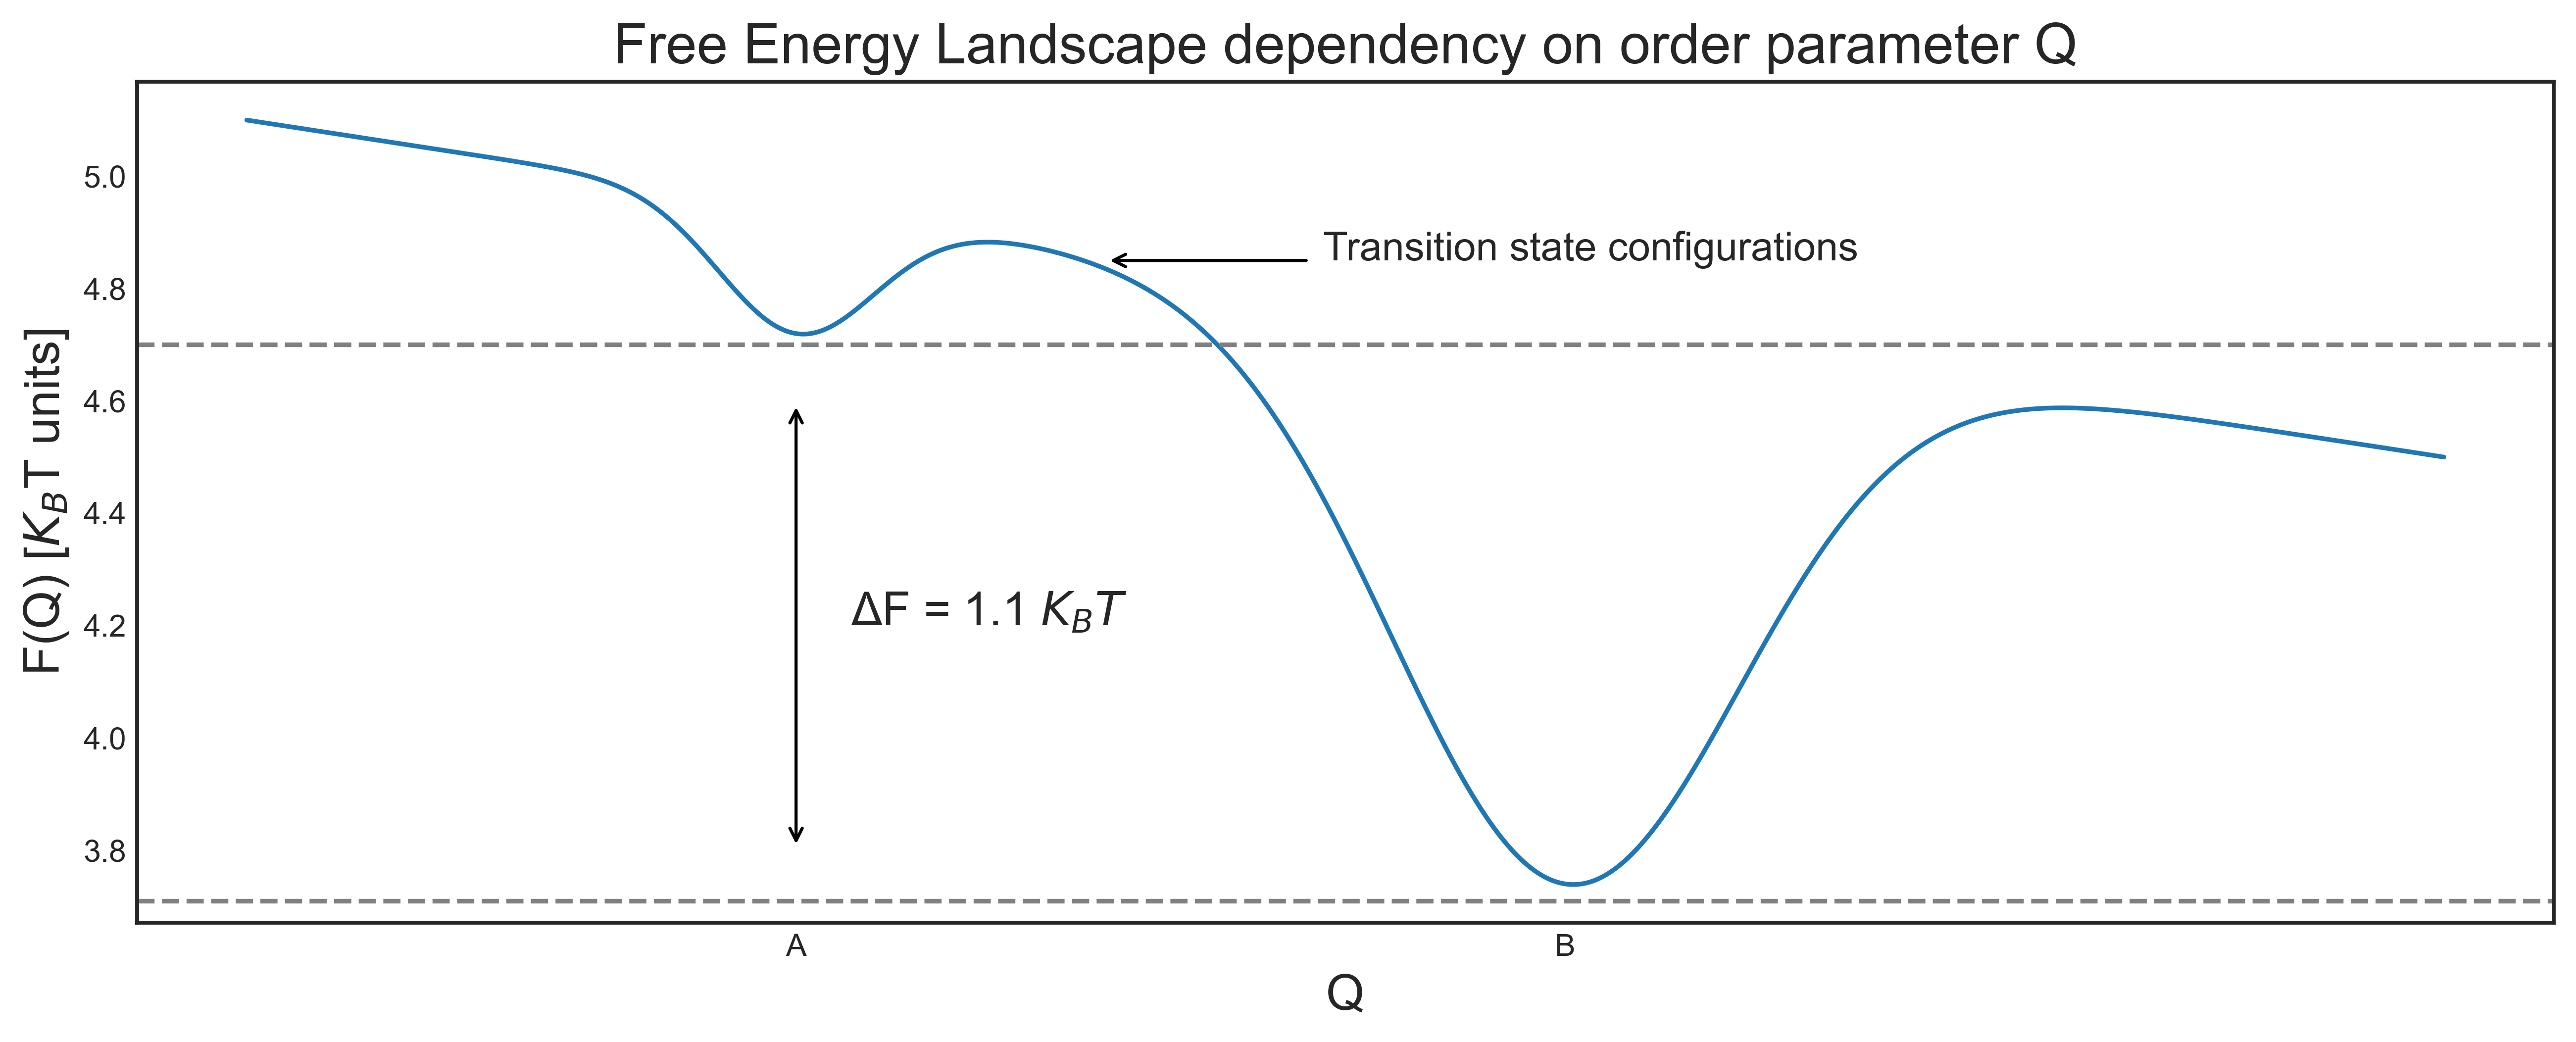
\includegraphics[width=1\textwidth]{imgs/FEL_Q.png}
\caption{Sketch of the Free energy landscape with the calculated difference between $F_A$ and $F_B$.The values displayed for F are arbitrary.The lower the value of F for a certain state, the more likely it is that the system is in that state.}
\label{img:walks}
\end{figure}
\subsection{Averages}
\textit{In this exercise you replaced ensemble averages with another type of averages: define both of them mathematically. What are the conditions for the two types to give the same results? Give a couple of examples of physical experiments where these conditions hold, and a couple where they do not hold.}

\subsection*{Solution}
In the exercise, averages over time are used to assume statistical properties that are obtained from averages made over the ensembles. The averages over time are calculated with arithmetic means on the properties of \textbf{one system} at different times of observation for a given long experiment, while the ensemble averages are calculated as avergaes of the observed property on the assumption of \textbf{multiple systems} for a given time without any kind of relationship with the time of evolution (causal disconnection and independence between the states of the system). These averages are equivalent in  \textbf{ergodic systems}, in which it is assumed that any trajectory (temporal evolution from an initial point) will visit all the possible states of the system given a sufficiently long observation time. It can be inferred that an arithmetic mean for the observed property on the points of the phase space visited by a single system trajectory (all of them) is equivalent to the average value obtained by taking into account all possible systems.

Applied to, for example, a system of many particles, it is considered equivalent to take the temporal average of a certain property for a single particle in a sufficiently long observation time, to take the average of said property for all the particles at a certain instant. The greater the number of (indistinguishable) particles,  it is mor accurate to say that both averages are equivalent following the  \textbf{ergodic hypothesis}.

Another relevant condition to have the equivalence between the averages is that they must be  \textbf{stationary processes}. This means that the probabilities associated with the observed properties should not change according to time translation. If this is not fulfilled, observing a single system over a long period is not equivalent to observing all systems for a certain time, since the properties of the systems are different depending on the time that it is chosen to observe. It is important to note that  \textbf{not all stationary processes are associated with ergodic systems, but ergodic systems must be stationary processes}.
\subsubsection*{Mathematical descriptions}
For time averages, the properties to be measured at different instants of time are taken into account for the same system $S$. Lets asume an observable $A$ present in the properties of the $i$-th system (starting in the point $x_o$ at $t_o$ )that is measured $n$ times over a given observation time $T$ :
\begin{equation}
    \hat{A_t}(S)  = \frac{1}{n}\sum_{t = 0}^{n-1} A(x_t)  
\end{equation}
This under the premise that $t_o < t_1 < t_2 < \ldots < t_{n-1 < T}$\\
For the ensemble average we have an ensemble composed by N systems, and at a given time the properties of all systems $s_i$ are observed and averaged.
\begin{equation}
     \hat{A_e}(S)  = \frac{1}{N}\sum_{i = 1}^{N} A(s_i) 
\end{equation}

The systems are equivalent when we have large observation times for $A_t$ and a large number of systems for $A_e$.
\subsubsection*{Examples}
An example of a non-ergodic system is the unbiased random walk, for which the temporal average of the displacement of a single walk is an erratic and random value, but for many systems the average displacement is 0. Other example is playing billard in an eliptical table, that has some initial states where despite all the possible collisions they cannot reach certain areas of the table. \\
An example of an ergodic system is the toss of a coin. By flipping the coin many times (with results 1 or 0), the average is eventually 1/2 for a long observation time. If many coins are picked and tossed at the same time, the average of the outcomes also tends to 1/2. Other good example is the ideal gas in a box, where it is assumed that after a long observation times, all accesible states are visited by the system in the phase space.
\subsection{Poison's law}
\textit{In general, rare transitions between metastable states are well described by Poisson's probability law: why? Compute the mean and the standard deviation of the first passage time (the time we have to wait to observe a transition from one metastable state to another one), considering that its probability density is given by the probability to observe zero jumps between 0 and t multiplied by the probability to observe one jump between t and t + dt.}
\subsection*{Solution}
The Poisson distribution is valid for the case of rare state transitions as it meets the following premises:
\begin{itemize}
    \item A state transition can occur any number of times in a given time interval.
    \item A transition event is independent of other past transition events.
    \item The rate of ocurrance of the transition event remains constant over time.
    \item a longer observation time proportionally implies more observed transition envents.
\end{itemize}
The Poisson distribution that describes \textit{"observing 0 transitions between time 0 and t"} is
\begin{equation}
    P_o(r) = e^{-rt}
\end{equation}
where $r$ is the observed rate of trnasitions present in a period of time. I calculated this rate as 14/40 given that ther are 14 timesteps corresponding to a transition in an interval of observation of 40 timesteps.\\
The Poisson distributioon for observing an event in the next $\delta_t$ after t is
\begin{equation}
    P_1(r) = r\delta_t e^{-r\delta_t}
\end{equation}
The probability distribution for the first passage time is given by the product f the two distributions, but
as $\delta_t \to 0$ , I can expand as
\begin{equation}
    P(r) =e^{-rt} \left(r\delta_t e^{-r\delta_t}\right)  = e^{-rt} \left(r\delta_t - \left(r\delta_t \right)^2 + \mathcal{O}(\delta_t^3)\right) \approx r\delta_t e^{-rt}
\end{equation}
Form this poisson distribution the properties of mean and standar deviation can be inferred as:

\begin{equation}
    \mu_p \approx r = 0.35
\end{equation}
\begin{equation*}
 \sigma_p \approx = \sqrt{r} = 0.59
\end{equation*}

\newpage

\section{Scientific articles}
\subsection*{Solution}
\textbf{Chosen Article: } \textit{S.K. Ma, Calculation of Entropy from Data of Motion, Journal of Statistical
Physics, Vol. 26, No. 2 (1981) } \cite{entropy_1981}
\subsection{Introduction and concepts}
The paper proposes to use an \textbf{ergodic approach} to calculate the entropy, among other thermodynamic properties of a system, from the trajectory that said system travels in \textbf{phase space}. This way of approaching the problem from the measurements of the system takes into account a \textbf{detailed history} of said trajectory over a considerable period of time to numerically calculate said quantities. As will be discussed later in this analysis, the conclusions made from a familiar example, such as an Ising kinetic model, allow corroborating the theoretical assumptions made regarding the reduction to \textbf{uncorrelated subsystems} within the assembly, as well as the validity of the numerical approximation with respect to the analytical calculation of the observed properties of the system in \textbf{thermodynamic equilibrium}. Another interesting result is the analysis of the nature of the \textbf{metastable states} and their influence on the trajectories of the phase space, as well as the study of the \textbf{relaxation times} that are defined for the system.

\subsubsection{Mechanical and Ensemble Approach}
The perspective of the analysis is established from two points of view: the \textbf{mechanical view}, which takes into account the trajectory in the phase space and history of the system to make conclusions regarding its thermodynamic properties, and the \textbf{ensemble view}, which interprets the system as a Gibbs ensemble for which a region in phase space is defined that depends on the properties of the entire system, and so do the thermodinamic properties. \\
The \textbf{ensemble view} requires the mathematical formulation of the system as a defined ensemble and its thermodynamic properties are derived from the representation of the ensemble in the phase space as a hypervolume of many (even infinite) possible subsystems, a volume that moves into a restricted region of the phase space following certain conservation properties (Liouville's Theorem). This makes the analysis of phase space and thermodynamic properties \textbf{independent of time}. This point of view requires defining the type of ensemble to be treated, which depends on the conserved quantities of the system and its boundary conditions. A weakness of this approach to the problem is the \texbf{ambiguity} that arises when dealing with metastable states.\\
On the other hand, the \textbf{mechanical view} analyzes how the system moves within the phase space with the evolution of the system for a considerable time of observation and concludes statistical properties from the history of states \textit{visited}. Note that to approach the problem from this perspective it is necessary to make some assumptions:

\begin{itemize}
    \item The observation time is \textbf{considerably longer} than the estimated relaxation time defined according to the system. This relaxation time is associated with the shortest relevant changes within the phase space.
    
    \item Separate states both spatially (within phase space) and/or temporally (several relaxation times) are \textbf{uncorrelated}.
    
    \item The states that are obtained over time are \textbf{randomly distributed} in the phase space so that the trajectory represents a random \textbf{sampling} of the space of possible configurations. This implies a direct correlation with the canonical and grand canonical ensemble where there is a uniform distribution in the phase space.
    
    \item If you have a system with many degrees of freedom (spatial dimensions, rotation, spin states, etc) and sseveral associated subsystems (particles, for example), it is almost certain that in the time considered for the trajectory, \textbf{not all} the possible microstates that the system can adopt will be \textit{visited}. This compromises the perspective of the ergodic system from which one starts.
    
    \item The latter implies that estimating the total number of possible states is \textit{apparently impossible}, however one of the main highlights of the article is how deduct this number from the \textbf{number of coincidences} that can be had in the phase space given a trajectory for a defined timelapse (the central method of the article is based on counting coincidences in the phase space to determine the entropy).
    
\end{itemize}
\subsubsection{The Coincidence counting method }
Given a system with $n$ sampling points along a trajectory in the phase space the expected number of coincidences $N_c$ among a number $\Gamma$ of possible microstates is given by
\begin{equation}
    N_c = \frac{n(n-1)}{2} \frac{1}{\Gamma}
\end{equation}
Having this in a set of $N_t = n(n-1)/2$ trials implies the existence of a coincidence probabilty per trial of $R = N_c/N_t = 1/\Gamma$. Given that the equation for entropy is
\begin{equation}
    S = \ln{\Gamma} = - \ln{R}
\end{equation}
This last statement is very important because it implies that if the number of coincidences $N_c$ and the number of trials  $n$ are known, then $\Gamma$, a counterpart of the system \textbf{partition function}, can be estimated. It also exposes one of the limitations of the method and that is that to have a good estimate of $\Gamma$ it is required that $N_c > 1$ and by extension $\sqrt{\Gamma} \leq n$.

\subsection{Interesting results and statements}
The article proposes a simulation method of a kinetic Ising system, in which there is a set of spins that have a coupling term with the other spins of the system. The probability of flipping for each spin depends on the temperature of the system and the coupling term with the other spins.  Tajectories in the phase space are simulated for many trials i.e. letting the system evolve step by step for a considerable time. The coincidences are counted as well as a cross section $V_s$ per state which determines the allowed similarity between two configurations to be considered as a coincidence. From this \textit{experiment} the article states:
\begin{itemize}

    \item Even for a relatively small Time for the trajectories, the estimate of the entropy missed for approximately 5\% the result form the analytical meyhod, which is amazing taking into account the simplicity of the method.
    \item metastable states can be seen as regions of the phase space in which the trajectory remains \textit{trapped} for relatively small periods of time. If the period of observation is short enough this states have well-defined thermodynamic properties. If the observation time is considerably long the system would leave this region eventually, so any metastable states under this macroscopic lense are not stabilities of defined properties anymore. This metastable states are easy to solve analytically in some cases, but when these regions get too complicated, the \textit{safety path} is to analyze the trajectories.
    \item Th third Law of Thermodynamics states that for a \textit{Zero Temperature}  the entropy vanishes. We know based on experiments that in this limit the entropy is nonzero because of the irreversibility of mestastable states. The coincidence counting method used on the Ising simulation agrees with the third law of thermodynamics since a Temperature approximating to Zero implies the \textbf{cessation of motion}. 
    \item Problems such as strong energy barriers limiting the phase space generate recurring metastates that, despite having very long observation times, prevent all possible system configurations from being explored. This takes away accuracy from the mechanical approach.
    \item states that are out of equilibrium are seen as \textbf{transitory states} between metastable states. These fluctuations are associated with a low frequency noise as a consequence of a constant flow and, relating this to cases of molecular configurations, it can be seen how these configurations that make up the transient flow are arranged as a \textit{cyclic path} between one or several metastable states. This would imply a \textbf{correlation} between separate microstates, \textbf{violating one of the initial assumptions} of the mechanical view. This can also be related to trajectories that are accessible only through a specific set of microstates.
\end{itemize}
The method of counting coincidences is a clever approach to the scenario of ergodic systems and is applicable to any system, even if its complexity is difficult to analyze mathematically, from which a detailed history of its trajectory in phase space can be obtained.  

% Computational Results
\printbibliography
\newpage
\begin{appendices}
\section{Additional Plots}
\textit{all plots available in The notebook referenced  in \cite{script_sims}}
\begin{figure}[h]
\centering

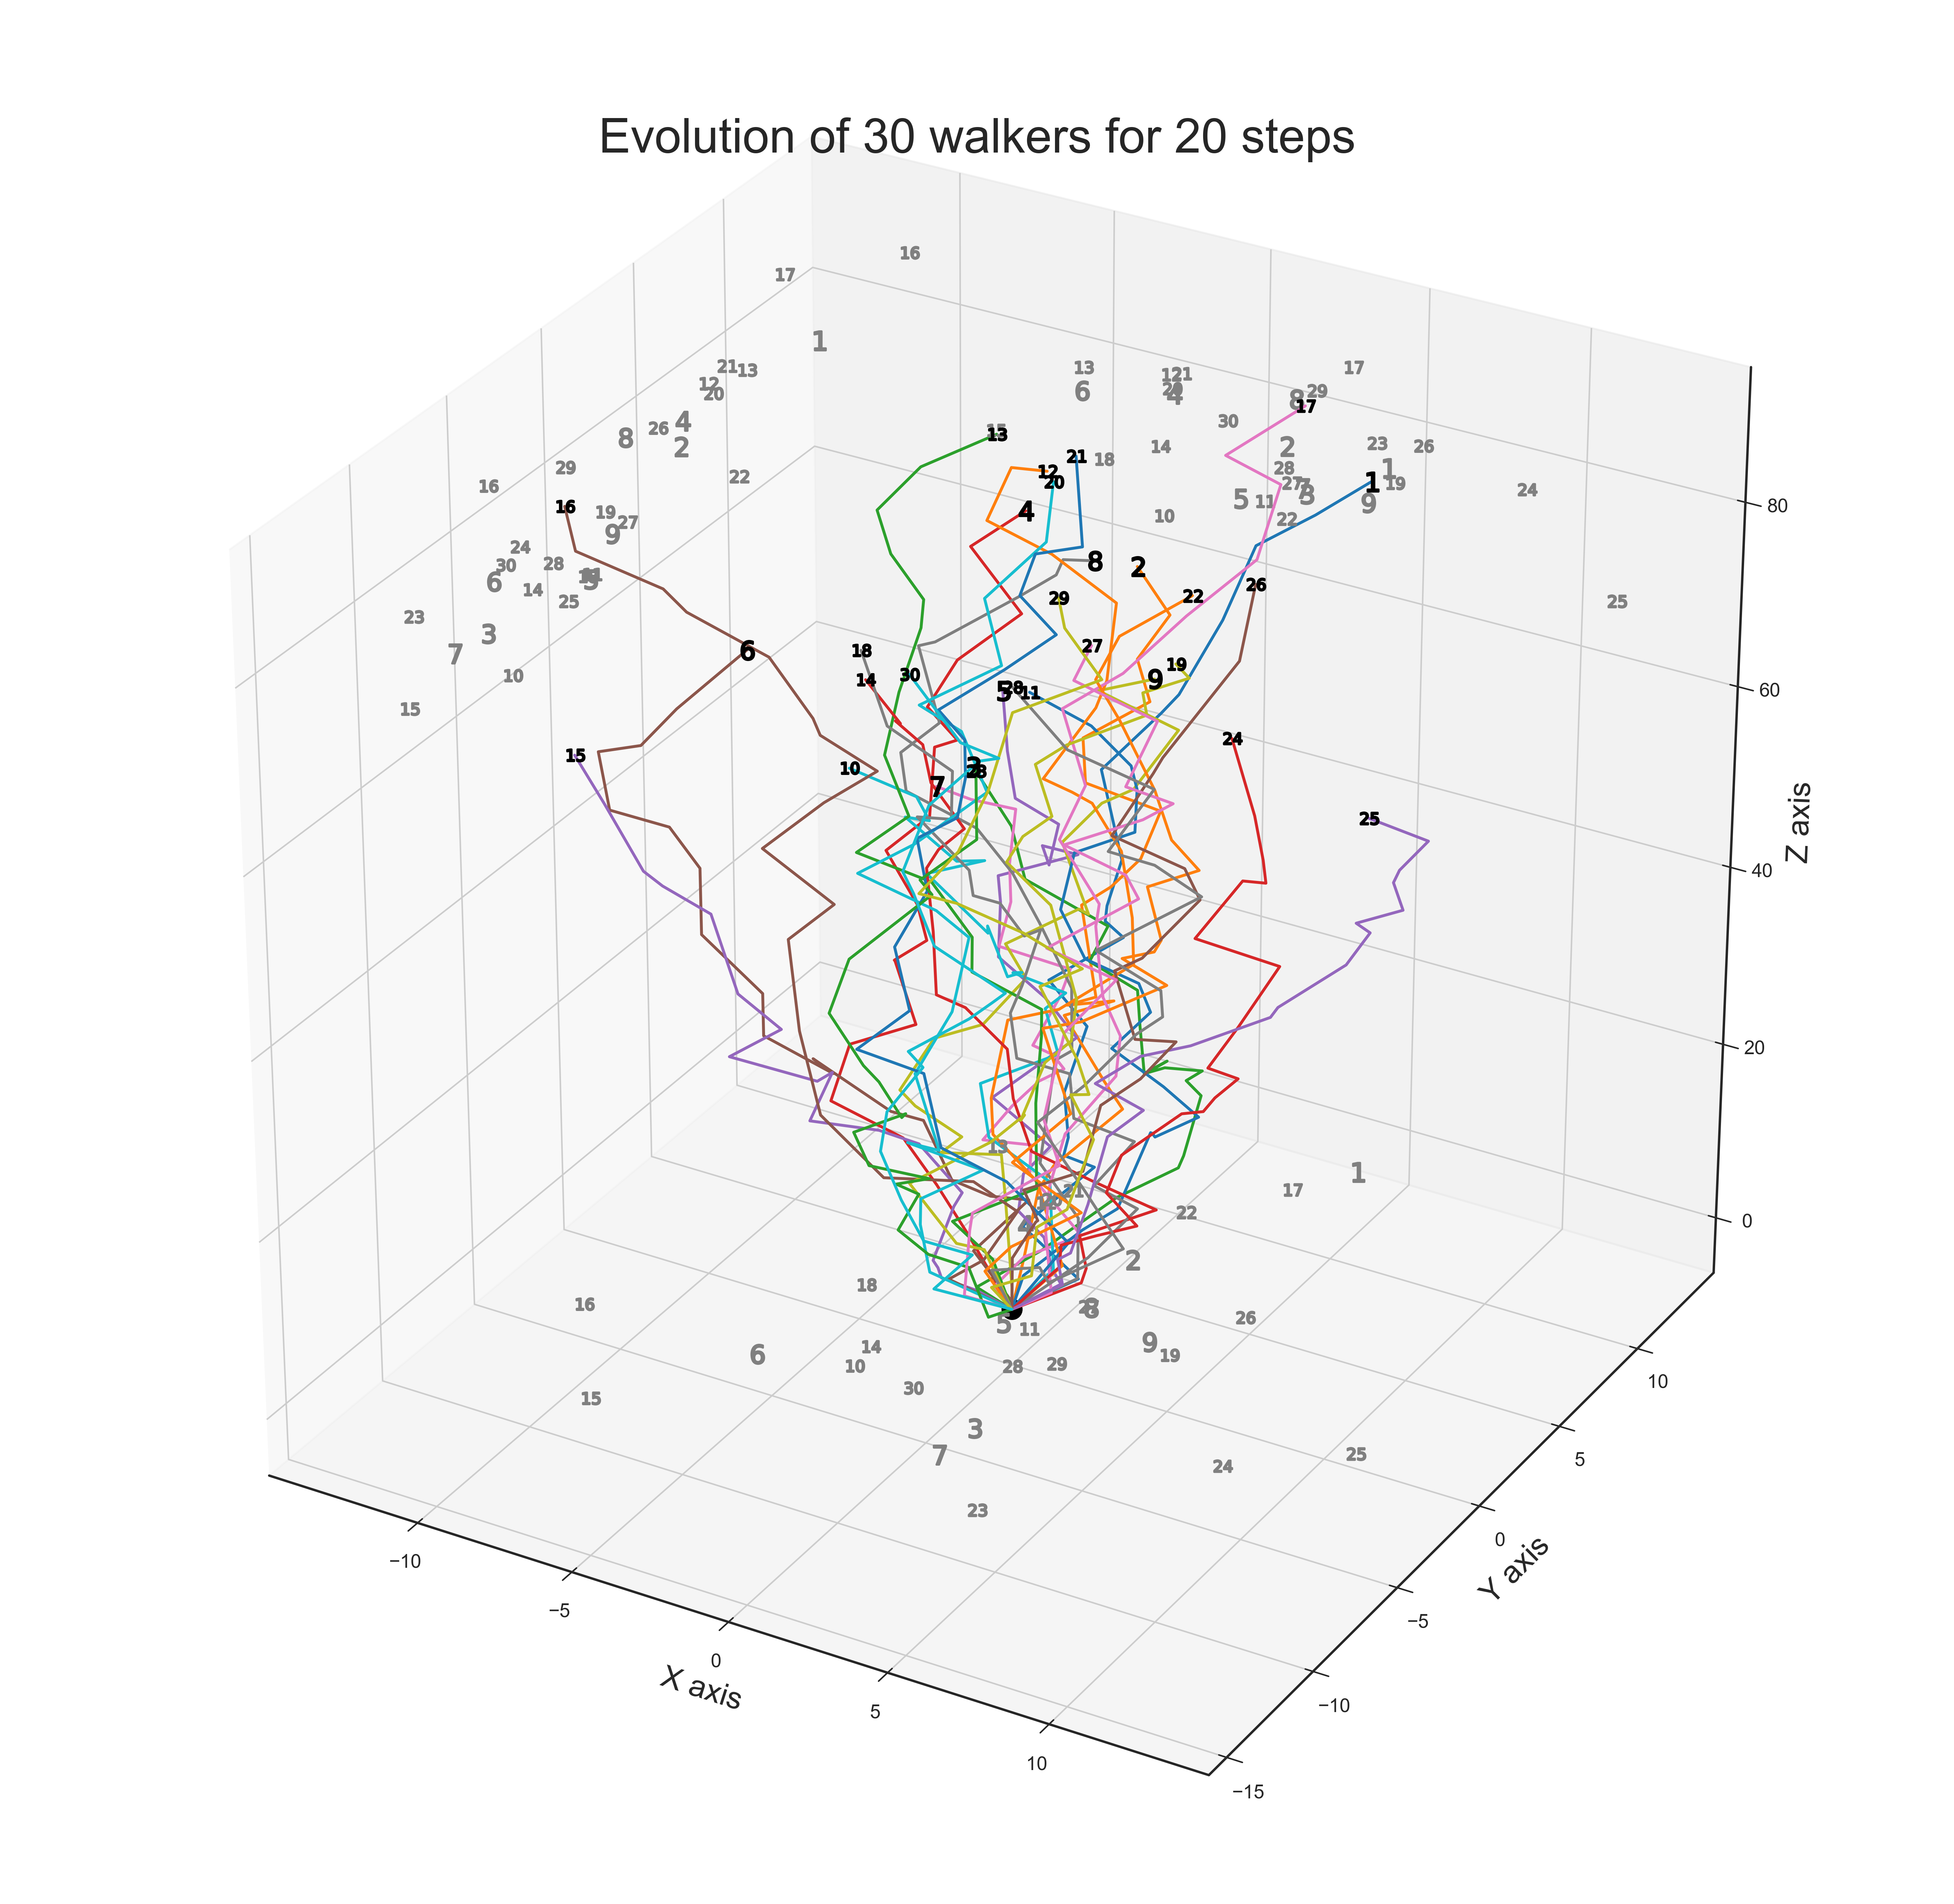
\includegraphics[width=1\textwidth]{imgs/walks.png}
\caption{Random walks in 3D following the given probaility ditributions for the steps. The labeled final positions are projected in the backgroud planes.}
\label{img:walks}
\end{figure}
\begin{figure}[h]
\centering

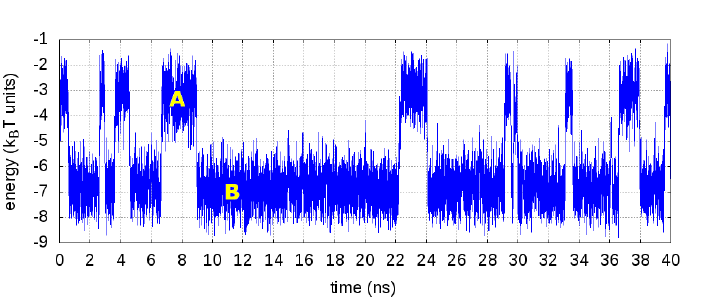
\includegraphics[width=1\textwidth]{imgs/hw_FELS.png}
\caption{Free Energy  Landscape available in the homework.}
\label{img:FELS}
\end{figure}

\begin{figure}[h]
\centering

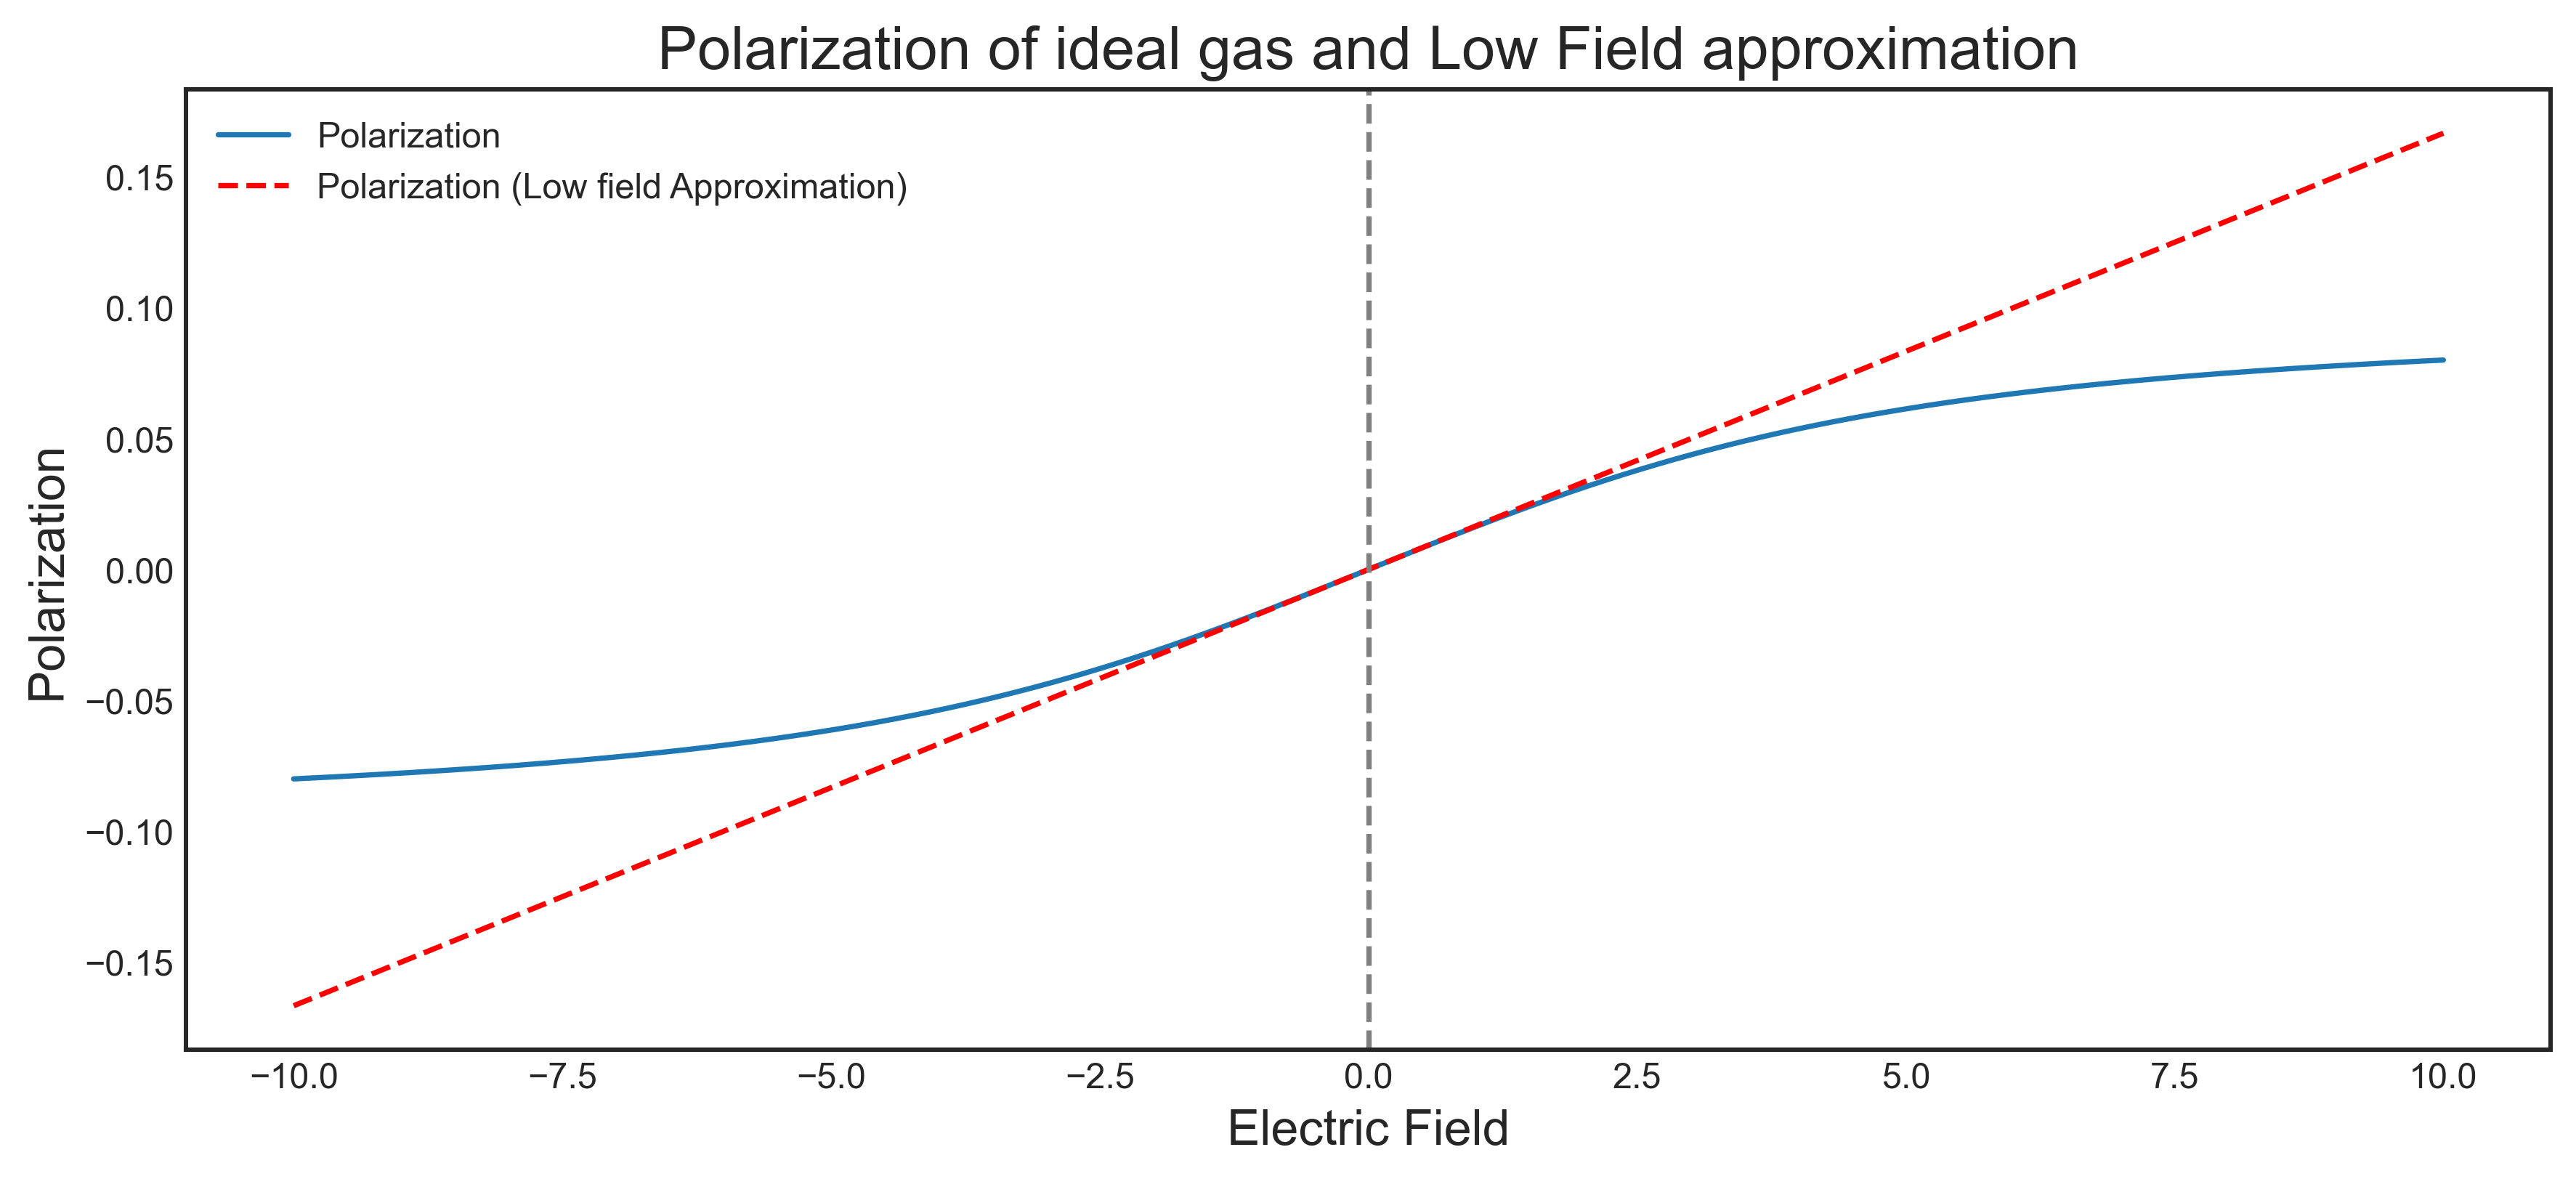
\includegraphics[width=1\textwidth]{imgs/polarization.png}
\caption{Polarization as a function of the field and the low field approximation where \textbf{E} is small}
\label{img:polarization}
\end{figure}
\end{appendices}

% \begin{table}
%     \centering
%     \begin{tabular}{rll}
%     & Name & Years \\
%     \hline
%     1 & Frosty & 1922-1930  \\
%     2 & Frosty II & 1930-1936 \\
%     3 & Wasky & 1946 \\
%     4 & Wasky II & 1947 \\
%     5 & Ski & 1954 \\
%     6 & Denali & 1958 \\
%     7 & King Chinook & 1959-1968\\
%     8 & Regent Denali & 1969 \\
%     9 & Sundodger Denali & 1981-1992 \\
%     10 & King Redoubt & 1992-1998 \\
%     11 & Prince Redoubt & 1998 \\
%     12 & Spirit & 1999-2008 \\
%     13 & Dubs I & 2009-2018 \\
%     14 & Dubs II & 2018-Present
%     \end{tabular}
%     \caption{UW mascots as described in \cite{washington_huskies}.}
%     \label{tab:mascots}
% \end{table}

% begin{figure}[tb] % t = top, b = bottom, etc.


% Summary and Conclusions
% \section{Summary and Conclusions}
% Add your summary and conclusions here.

% References


% Appendices
% \begin{appendices}

% % MATLAB Functions
% \section{MATLAB Functions}
% Add your important MATLAB functions here with a brief implementation explanation. This is how to make an \textbf{unordered} list:
% \begin{itemize}
%     \item \texttt{y = linspace(x1,x2,n)} returns a row vector of \texttt{n} evenly spaced points between \texttt{x1} and \texttt{x2}. 
%     \item \texttt{[X,Y] = meshgrid(x,y)} returns 2-D grid coordinates based on the coordinates contained in the vectors \texttt{x} and \texttt{y}. \text{X} is a matrix where each row is a copy of \texttt{x}, and \texttt{Y} is a matrix where each column is a copy of \texttt{y}. The grid represented by the coordinates \texttt{X} and \texttt{Y} has \texttt{length(y)} rows and \texttt{length(x)} columns.  
% \end{itemize}

% % MATLAB Codes
% \section{MATLAB Code}
% Add your MATLAB code here. This section will not be included in your page limit of six pages.

% \begin{listing}[h]
% \inputminted{matlab}{example.m}
% \caption{Example code from external file.}
% \label{listing:examplecode}
% \end{listing}

% \end{appendices}

\end{document}
